\documentclass{fenicsmanual}

\begin{document}

\fenicstitle{DOLFIN User Manual}
\fenicsauthor{Logg, Wells, et al.}
\fenicspackage{\textbf{\textsf{DOLFIN}}}{dolfin}
\fenicsimage{eps/dolfin.eps}

\maketitle

% This chapter is common to the DOLFIN and FFC manuals.

\addcontentsline{toc}{chapter}{About this manual}
\chapter*{About this manual}

This manual is currently being written. As a consequence, some sections
may be incomplete or inaccurate.

%------------------------------------------------------------------------------
\section*{Intended audience}

This manual is written both for the beginning and the advanced user.
There is also some useful information for developers. More advanced topics
are treated at the end of the manual or in the appendix.

%------------------------------------------------------------------------------
\section*{Typographic conventions}
\index{typographic conventions}

\begin{itemize}
\item
  Code is written in monospace (typewriter) \texttt{like this}.
\item
  Commands that should be entered in a Unix shell
  are displayed as follows:
  \begin{code}
    # ./configure
    # make
  \end{code}
  Commands are written in the dialect of the \texttt{bash} shell. For
  other shells, such as \texttt{tcsh}, appropriate translations may be
  needed.
\end{itemize}

%------------------------------------------------------------------------------
\section*{Enumeration and list indices}
\index{enumeration}
\index{indices}

Throughout this manual, elements $x_i$ of sets $\{x_i\}$ of size $n$
are enumerated from $i = 0$ to $i = n-1$. Derivatives in $\R^n$ are
enumerated similarly:
$\frac{\partial}{\partial x_0}, \frac{\partial}{\partial x_1},
 \ldots, \frac{\partial}{\partial x_{n-1}}$.

%------------------------------------------------------------------------------
\section*{Contact}
\index{contact}

Comments, corrections and contributions to this manual are most welcome
and should be sent to
\begin{code}
  \packagett{}-dev@fenics.org    
\end{code}

%\chapter{Introduction}

\fixme{Automation of CMM, FEniCS, purpose of DOLFIN: PSE for differential equations, C++ interface of
  FEniCS, etc}

%------------------------------------------------------------------------------
\section{The FEniCS project}
\index{FEniCS}
\index{automation}

\fixme{Automation of CMM, other components of \fenics{}}

%------------------------------------------------------------------------------
\section{The finite element method}
\index{finite element method}

\fixme{Automation of discretization}

%------------------------------------------------------------------------------
\section{Overview}

\fixme{Component diagram, user, module, kernel}

\fixme{Write about \texttt{real}, \texttt{uint}, namespace \texttt{dolfin}}

\input{chapters/quickstart.tex}
\input{chapters/linearalgebra.tex}
\chapter{The mesh}

\devnote{This chapter is just a quick write-up of the most basic
  functionality of the mesh library and will be expanded.}

% FIXME: Need to write about mesh.init()

\section{Basic concepts}

\subsection{Mesh}

A \emph{mesh} consists of \emph{mesh topology} and \emph{mesh geometry}.
These concepts are implemented by the classes \texttt{Mesh},
\texttt{MeshTopology} and \texttt{MeshGeometry}.

\subsection{Mesh entities}

% FIXME: Add some nice figures here

A \emph{mesh entity} is a pair $(d, i)$, where $d$ is the topological
dimension of the mesh entity and $i$ is a unique index of the mesh
entity. Mesh entities are numbered within each topological dimension
from $0$ to $n_d-1$, where $n_d$ is the number of mesh entities of
topological dimension $d$.

For convenience, mesh entities of topological dimension $0$ are
referred to as \emph{vertices}, entities of dimension $1$
\emph{edges}, entities of dimension $2$ \emph{faces}, entities of
\emph{codimension} $1$ \emph{facets} and entities of codimension $0$
\emph{cells}. These concepts are summarized in
Table~\ref{tab:entities,here}.

\begin{table}[htbp]
  \begin{center}
    \begin{tabular}{|l|c|c|}
      \hline
      Entity & Dimension & Codimension \\
      \hline
      Vertex & $0$       & -- \\
      Edge   & $1$       & -- \\
      Face   & $2$       & -- \\
      & & \\
      Facet  & --      &  $1$ \\
      Cell   & --      &  $0$ \\
      \hline
    \end{tabular}
    \caption{Named mesh entities.}
    \label{tab:entities,here}
  \end{center}
\end{table}

These concepts are implemented by the classes
\texttt{MeshEntity},
\texttt{Vertex},
\texttt{Edge},
\texttt{Face},
\texttt{Facet},
\texttt{Cell}.

\section{Mesh iterators}

Algorithms operating on a mesh
can often be expressed in terms of
\emph{iterators}. The mesh library provides the general iterator
\texttt{MeshEntityIterator} for iteration over mesh entities, as well
as the specialized mesh iterators
\texttt{VertexIterator},
\texttt{EdgeIterator},
\texttt{FaceIterator},
\texttt{FacetIterator} and
\texttt{Cell\-Iterator}.

The following code illustrates how to iterate over all incident
(connected) vertices of all vertices of all cells of a given mesh:
\begin{code}
for (CellIterator c(mesh); !c.end(); ++c)
  for (VertexIterator v0(*c); !v0.end(); ++v0)
    for (VertexIterator v1(*v0); !v1.end(); ++v1)
      cout << *v1 << endl;
\end{code}
This may alternatively be implemented using the general iterator
\texttt{MeshEntity\-Iterator} as follows:
\begin{code}
unsigned int dim = mesh.topology().dim();
for (MeshEntityIterator c(mesh, dim); !c.end(); ++c)
  for (MeshEntityIterator v0(*c, 0); !v0.end(); ++v0)
    for (MeshEntityIterator v1(*v0, 0); !v1.end(); ++v1)
      cout << *v1 << endl;
\end{code}

\section{Mesh functions}

A \texttt{MeshFunction} represents a discrete function that takes a
value on each mesh entity of a given topological dimension.
A \texttt{MeshFunction} may for example be used to store a global
numbering scheme for the entities of a (parallel) mesh, marking
sub domains or boolean markers for mesh refinement.

\section{Mesh refinement}

A mesh may be refined uniformly as follows:
\begin{code}
mesh.refine();
\end{code}
A mesh may also be refined locally by supplying a
\texttt{MeshFunction} with boolean markers for the cells that should
be refined.

\section{Working with meshes}

\subsection{Reading a mesh from file}

A mesh may be loaded from a file, either by specifying the file name
to the constructor of the class \texttt{Mesh}:
\begin{code}
Mesh mesh("mesh.xml");
\end{code}
or by creating a \texttt{File} object and streaming to a
\texttt{Mesh}:
\begin{code}
File file("mesh.xml");
Mesh mesh;
file >> mesh;
\end{code}
A mesh may be stored to file as follows:
\begin{code}
File file("mesh.xml");
Mesh mesh;
file << mesh;
\end{code}

The \dolfin{} mesh XML format has changed in \dolfin{} version
0.6.3. Meshes in the old XML format may be converted to the new XML
format using the script \texttt{dolfin-convert} included in the
distribution of \dolfin{}. For instructions, type
\texttt{dolfin-convert --help}.

\subsection{Extracting a boundary mesh}

For any given mesh, a mesh of the boundary of the mesh (if any) may be
created as follows:
\begin{code}
BoundaryMesh boundary(mesh);
\end{code}
A \texttt{BoundaryMesh} is itself a \texttt{Mesh} of the same
geometrical dimension and has the topological dimension of the mesh
minus one.

The computation of a boundary mesh may also provide mappings from the
vertices of the boundary mesh to the corresponding vertices in the
original mesh, and from the cells of the boundary mesh to the
corresponding facets of the original mesh:
\begin{code}
MeshFunction<unsigned int> vertex_map,
MeshFunction<unsigned int> cell_map;
BoundaryMesh boundary(mesh, vertex_map, cell_map);
\end{code}

\subsection{Built-in meshes}

\dolfin{} provides functionality for creating simple meshes, such as
the mesh of the unit square and the unit cube. The following code
demonstrates how to create a $16\times 16$ triangular mesh of the unit square
(consisting of $2\times 16\times 16 = 512$ triangles) and a
$16\times 16\times 16$ tetrahedral mesh of the unit cube (consisting
of $6\times 16\times 16\times 16 = 24576$ tetrahedra):
\begin{code}
UnitInterval mesh1D(16);
UnitSquare mesh2D(16, 16);
UnitCube mesh3D(16, 16, 16);
\end{code}

\devnote{We could easily add other built-in meshes, like the unit disc,
  the unit sphere, rectangles, blocks etc.
  Any contributions are welcome.}

\subsection{Creating meshes}

Simplicial meshes (meshes consisting of intervals, triangles or
tetrahedra) may be constructed explicitly by specifying the
cells and vertices of the mesh. A specialized interface for creating
simplicial meshes is provided by the class \texttt{MeshEditor}.
The following code demonstrates how to create a very simple mesh
consisting of two triangles covering the unit square:
\begin{code}
Mesh mesh;
MeshEditor editor(mesh, CellType::triangle, 2, 2);
editor.initVertices(4);
editor.initCells(2);
editor.addVertex(0, 0.0, 0.0);
editor.addVertex(1, 1.0, 0.0);
editor.addVertex(2, 1.0, 1.0);
editor.addVertex(3, 0.0, 1.0);
editor.addCell(0, 0, 1, 2);
editor.addCell(1, 0, 2, 3);
editor.close();
\end{code}
Note that the \dolfin{} mesh library is not specialized to simplicial
meshes, but supports general collections of mesh entities. However,
tools like mesh refinement and mesh editors are currently only
available for simplicial meshes.

\input{chapters/functions.tex}
\chapter{Ordinary differential equations}

\devnote{This chapter needs to be written. In the meantime, checkout the demos
  in \texttt{src/demo/ode/} and the base class \texttt{ODE}.}


% FIXME: Mono-adaptive, multi-adaptive, ODE base class, simple example,
% FIXME: error control, adaptivity, complex ODE, implicit, homotopies

\chapter{Partial differential equations}
\label{sec:pde}
\index{partial differential equations}

\devnote{This chapter needs to be written. In the meantime, look at the demos
  in \texttt{src/demo/pde/}.}

%\devnote{This chapter is incomplete and inaccurate and needs to be updated.
%In the meantime, look at the demos in \texttt{src/demo/pde/}.}
%
%\dolfin{} provides a general interface for defining a partial differential 
%equation (PDE) in variational form. The variational form is compiled 
%with \ffc{}, which generates code for the assembly of a matrix and a 
%vector, corresponding to the discretization of the PDE with a user-defined  
%finite element method (FEM), where the basis functions of the FEM space 
%are constructed using \fiat{}. 
%
%\section{Boundary value problems}
%
%As a prototype of a boundary value problem in $\Bbb{R}^d$ we consider the 
%scalar Poisson equation with homogeneous Dirichlet boundary conditions 
%\begin{eqnarray}
%-\Delta u(x)&=&f(x) \quad x\in \Omega \subset \Bbb{R}^d \label{pde:poisson:strong} \\
%u(x)&=&0 \quad x\in \partial \Omega. \nonumber  
%\end{eqnarray}
%
%\section{Variational formulation}
%
%A variational formulation of (\ref{pde:poisson:strong}) takes the form: 
%find $u\in V$ such that  
%\begin{equation}\label{pde:poisson:weak}
%a(v,u)=L(v) \quad \forall v\in \hat V, 
%\end{equation}
%where $a(\cdot,\cdot):\hat V\times V\rightarrow \Bbb{R}$ is a bilinear form 
%acting on $\hat V \times V$, with $\hat V$ and $V$ the {\em test space} and {\em trial space} 
%respectively, defined by 
%\begin{equation}
%a(v,u)=\int_{\Omega} \nabla v \cdot \nabla u ~dx 
%=\int_{\Omega} \frac{\partial v}{\partial x_i} \frac{\partial u}{\partial x_i} ~ dx,  
%\end{equation}
%where we employ tensor notation so that the double index $i$ means summation from $i=1,...,d$, 
%and $L(\cdot):\hat V\rightarrow \Bbb{R}$ is a linear form acting on the test space $\hat V$,  
%defined by 
%\begin{equation}
%L(v)=\int_{\Omega} v f ~dx.  
%\end{equation}
%For this problem we typically use $V=\hat V=H^1_0(\Omega)$, with $H^1_0(\Omega)$ 
%the standard Sobolev space of square integrable functions with also their first 
%derivatives square integrable (in the Lebesgue sense), 
%with the functions being zero on the boundary (in the sense of traces).
%
%The FEM method for (\ref{pde:poisson:weak}) is now: 
%find $U\in V_h$ such that  
%\begin{equation}\label{pde:poisson:fem}
%a(v,U)=L(v) \quad \forall v\in \hat V_h, 
%\end{equation}
%where $V_h\subset V$ and $\hat V_h\subset \hat V$ are finite dimensional 
%subspaces of dimension $M$. 
%The finite element spaces $V_h,\hat V_h$ are characterized by their sets of basis 
%functions $\{\varphi_i\}_{i=1}^M,\{\hat \varphi_i\}_{i=1}^M$. 
%The FEM method (\ref{pde:poisson:fem}) is thus specified by the 
%variational form and the basis functions of $V_h$ and $\hat V_h$.

% \section{Finite elements and \fiat{}}

% Finite element basis functions in \dolfin{} are defined using \fiat{}, 
% which supports the generation of arbitrary order Lagrange finite 
% elements on lines, triangles, and tetrahedra. 
% Upcoming versions of \fiat{} will also support Hermite and nonconforming 
% elements as well as H(div) and H(curl) elements such as Raviart-Thomas and Nedelec.

% \section{Compiling the variational form with \ffc{}}

% In \dolfin{} a PDE is defined in variational form using tensor notation 
% in a \texttt{.form} file, which is compiled using \ffc{}. 

% In the language of \ffc{}, with $V_h=\hat V_h$ the space of piecewise linear Lagrange 
% finite elements on a tetrahedral mesh, (\ref{pde:poisson:fem}) is defined as:  
% \begin{code}
% element = FiniteElement("Lagrange", "tetrahedron", 1)

% v = BasisFunction(element)
% u = BasisFunction(element)
% f = Function(element)

% a = v.dx(i)*u.dx(i)*dx
% L = v*f*dx
% \end{code}
% where \texttt{*dx} signifies integration over the domain $\Omega$, and 
% the finite element space is constructed using \fiat{}. 
% \dolfin{} is not communicating directly with \fiat{}, but only through 
% \ffc{} in the definition of the variational form in the \texttt{.form} file.  

% Compiling the \texttt{.form} file with 
% \begin{code}
% # ffc Poisson.form
% \end{code}
% generates a file \texttt{Poisson.h}, containing classes for 
% the bilinear form $a(\cdot,\cdot)$ and the linear form $L(\cdot)$, 
% and classes for the finite element spaces $V_h$ and $\hat V_h$. 

% \section{Element matrices and vectors} 

% The element matrices and vectors for a given cell may be factored 
% into two tensors, with one tensor depending on the geometry of the cell, 
% and the other tensor only involving integration of products of 
% basis functions and their derivatives over the reference element.  

% For efficiency in the computation of the element matrices 
% and vectors, \ffc{} precomputes the tensors that are independent of 
% the geometry of a certain cell. 

% \section{Assemble matrices and vectors}

% The class \texttt{FEM} automates the assembly algorithm, constructing a linear 
% system of equations from a PDE, 
% given in the form of a variational problem (\ref{pde:poisson:weak}), 
% with a bilinear form $a(\cdot,\cdot)$ and a linear form $L(\cdot)$. 

% The classes \texttt{BilinearForm} and \texttt{LinearForm} are automatically 
% generated by \ffc{}, and to assemble the corresponding matrix and vector for 
% the Poisson problem (\ref{pde:poisson:weak}) with source term $f$, we write:  
% \begin{code}
% Poisson::BilinearForm a;
% Poisson::LinearForm L(f);

% Mesh mesh; 
% Mat A;
% Vec b;

% FEM::assemble(a,L,A,b,mesh);
% \end{code}

% In the \texttt{assemble()} function the element matrices and vectors are 
% computed by calling the function \texttt{eval()} in the classes 
% \texttt{Bilinearform} and \texttt{Linearform}. 
% The \texttt{eval()} functions at a certain element in the assembly algorithm 
% take as argument an \texttt{AffineMap} object, 
% describing the mapping from the reference element to the actual element, 
% by computing the Jacobian $J$ of the mapping (also $J^{-1}$ and $det(J)$ 
% are computed).  

% \section{Specifying boundary conditions and data}

% The boundary conditions are specified by defining a new subclass 
% of the class \texttt{BoundaryCondition}, 
% which we here will name \texttt{MyBC}: 
% \begin{code}
%   class MyBC : public BoundaryCondition
%   \{
%     const BoundaryValue operator() (const Point& p)
%     \{
%       BoundaryValue value;
%       if ( std::abs(p.x - 0.0) < DOLFIN_EPS ) value = 0.0;
%       if ( std::abs(p.x - 1.0) < DOLFIN_EPS ) value = 0.0;
%       if ( std::abs(p.y - 0.0) < DOLFIN_EPS ) value = 0.0;
%       if ( std::abs(p.y - 1.0) < DOLFIN_EPS ) value = 0.0;
%       if ( std::abs(p.z - 0.0) < DOLFIN_EPS ) value = 0.0;
%       if ( std::abs(p.z - 1.0) < DOLFIN_EPS ) value = 0.0;
%         return value;
%     \}
%   \};
% \end{code}
% where we have assumed homogeneous Dirichlet boundary conditions for the 
% unit cube. 
% We only need to specify the boundary conditions explicitly on the
% Dirichlet boundary. On the remaining part of the boundary, 
% homogeneous Neumann boundary conditions are automatically imposed 
% weakly by the variational form. 

% The boundary conditions are then imposed as an argument to  
% the \texttt{assemble()} function: 
% \begin{code}
% MyBC bc; 
% FEM::assemble(a,L,A,b,mesh,bc);
% \end{code}

% There is currently no easy way to impose non-homogeneous
% Neumann boundary conditions or other combinations of boundary
% conditions. This will be added to a future release of \dolfin{}.

% The right-hand side $f$ of (\ref{pde:poisson:strong}) is similarly 
% specified by defining a new subclass of \texttt{Function}, which we
% here will name \texttt{MyFunction}, and overloading the evaluation
% operator: 
% \begin{code}
%   class MyFunction : public Function
%   \{
%     double operator() (const Point& p) const
%     \{
%       return p.x*p.z*sin(p.y);
%     \}
%   \};
% \end{code}
% with the source $f(x, y, z) = x z \sin(y)$. 

% \section{Initial value problems}

% A time dependent problem has to be discretized in time manually, 
% and the resulting variational form is then discretized in space 
% using \ffc{} similarly to a stationary problem, with the solution 
% at previous time steps provided as data to the \texttt{form} file. 

% For example, the form file \texttt{Heat.form} for the heat equation 
% discretized in time with the implicit Euler method, takes the form: 
% \begin{code}
% v           = BasisFunction(scalar) # test function
% u1          = BasisFunction(scalar) # value at next time step
% u0          = Function(scalar)      # value at previous time step
% f           = Function(scalar)      # source term
% k           = Constant()            # time step

% a = v*u1*dx + k*v.dx(i)*u1.dx(i)*dx 
% L = v*u0*dx + v*f*dx 
% \end{code}
% which generates a file \texttt{Heat.h} when compiled with \ffc{}. 
% To initializations the corresponding forms we write:  
% \begin{code}
% double k;                  // time step
% Vector x0;               // vector containing dofs for u0
% Function u0(x0, mesh);   // solution at previous time step 

% Heat::BilinearForm a(k);
% Heat::LinearForm L(u0,f,k);
% \end{code}

\chapter{Nonlinear solver}
\index{nonlinear solver}

\devnote{This chapter is currently being written\ldots}

\dolfin{} provides tools for solving nonlinear equations of the form
\begin{equation}
  F(u) = 0
\end{equation}
where $F: \mathbb{R}^{n} \rightarrow \mathbb{R}^{n}$. The nonlinear solvers are
based on Newton's method and utilise functions from PETSc \cite{www:petsc}.    

To use the nonlinear solver, a nonlinear function must be defined. The nonlinear
solver is then initialised with this function and a solution computed.



\section{Nonlinear functions}
\index{NonlinearFunction}

To solve a nonlinear problem, the user must defined a class which . The class 
should be derived from the \dolfin class \texttt{NonlinearFunction}. The class 
should contain the necessary functions to form the function $F(u)$ and the 
Jacobian matrix  $J = \partial F / \partial u$. The precise form of the user 
defined class will depend on the PDE being solved and the numerical method.
The structu of a user defined class \texttt{MyNonlinearFunction} is shown below.
\begin{code}
class MyNonlinearFunction : public NonlinearFunction
\{
  public: 
  
    // Constructor 
    MyNonlinearFunction() : NonlinearFunction()\{\}
  
    // Compute F(u) 
    void F(Vector\& b, const Vector\& x)
    \{
      // Insert F(u) into the vector b 
    \}

    // Compute J
    void J(Matrix\& A, const Vector\& x)
    \{
      // Insert the Jacobian into the matrix A 
    \}

    dolfin::uint size()
    \{      
      // Return the dimension of the Jacobian matrix 
    \}

    dolfin::uint nzsize()
    \{      
      // Return the maximum number of zeroes per row of the Jacobian
    \}

  private:
    // Pointers to objects with which F(u) is defined
\};
\end{code}


\section{Newton solver}
\index{Newton's method}
\index{NewtonSolver}

\subsection{Linear solver}

\subsection{Application of Dirichlet boundary conditions}

The application of inhomogenuous Dirichlet boundary conditions in the context
of a Newton solver requires particular attention.



\subsection{Newton solver parameters}

\subsection{Application of Dirichlet boundary conditions}


\section{Incremental Newton solver}


\input{chapters/io.tex}
\chapter{The log system}
\index{log system}

\dolfin{} provides provides a simple interface for uniform handling of
log messages, including warnings and errors. All messages are
collected to a single stream, which allows the destination and
formatting of the output from an entire program, including the
\dolfin{} library, to be controlled by the user.

%------------------------------------------------------------------------------
\section{Generating log messages}
\index{\texttt{info()}}
\index{\texttt{cout}}
\index{\texttt{endl}}

Log messages can be generated using the function
\texttt{info()} available in the \texttt{dolfin} namespace:
\begin{code}
void info(std::string format, ...);
\end{code}
which works similarly to the standard C library function \texttt{printf}.
The following examples illustrate the usage of
\texttt{info()}:
\begin{code}
info("Solving linear system.");
info("Size of vector: \%d.", x.size());
info("R = \%.3e (TOL = \%.3e)", R, TOL);
\end{code}

As an alternative to \texttt{info()}, \dolfin{} provides a C++
style interface to generating log messages. Thus, the above examples
can also be implemented as follows:
\footnotesize
\begin{code}
cout << "Solving linear system." << endl;
cout << "Size of vector: " << x.size() << "." << endl;
cout << "R = " << R << " (TOL = " << TOL << ")" << endl;
\end{code}
\normalsize
Note the use of \texttt{dolfin::cout} and
\texttt{dolfin::endl} from the \texttt{dolfin} namespace,
corresponding to the standard standard \texttt{std::cout} and
\texttt{std::endl} in namespace \texttt{std}. If log messages are
directed to standard output (see below), then \texttt{dolfin::cout}
and \texttt{std::cout} may be mixed freely.

Most classes provided by \dolfin{} can be used together with
\texttt{dolfin::cout} and \texttt{dolfin::endl} to display short
informative messages about objects:
\begin{code}
Matrix A(10, 10);
cout << A << endl;
\end{code}
To display detailed information for an object,  use the member function
\texttt{disp()}:
\begin{code}
Matrix A(10, 10);
A.disp();
\end{code}
Use with caution for large objects. For a \texttt{Matrix}, calling
\texttt{disp()} displays all matrix entries.

%------------------------------------------------------------------------------
\section{Warnings and errors}
\index{warnings}
\index{errors}
\index{\texttt{warning()}}
\index{\texttt{error()}}

Warnings and error messages can be generated using the functions
\begin{code}
warning(std::string format, ...);
error(std::string format, ...);
\end{code}
Once an error is encountered, the program throws an exception.

%------------------------------------------------------------------------------
\section{Debug messages and assertions}
\index{debugging}
\index{assertions}
\index{\texttt{dolfin\_debug()}}
\index{\texttt{dolfin\_assert()}}

The macro \texttt{dolfin\_debug()} works similarly to
\texttt{info()}:
\begin{code}
dolfin_debug(message);
\end{code}
but in addition to displaying the given message, information is printed about
the location of the code that generated the debug message (file,
function name and line number).

Note that in order to pass formatting strings and additional arguments
with debug messages, the variations \texttt{dolfin\_debug1()},
\texttt{dolfin\_debug2()} and so on, depending on the number of
arguments, must be used.

Assertions can often be a helpful programming tool. Use assertions
whenever you assume something about about a variable in your code,
such as assuming that given input to a function is valid. \dolfin{}
provides the macro \texttt{dolfin\_assert()} for creating assertions:
\begin{code}
dolfin_assert(check);
\end{code}
This macro accepts a boolean expression and if the expression
evaluates to false, an error message is displayed, including the
file, function name and line number of the assertion, and a
segmentation fault is raised (to enable easy attachment to a
debugger). The following examples illustrate the use of
\texttt{dolfin\_assert()}:
\begin{code}
dolfin_assert(i >= 0);
dolfin_assert(i < n);
dolfin_assert(cell.type() == Cell::triangle);
dolfin_assert(cell.type() == Cell::tetrahedron);
\end{code}
Note that assertions are only active when compiling
\dolfin{} and your program with \texttt{DEBUG} defined (configure
option \texttt{--enable-debug} or compiler flag \texttt{-DDEBUG}).
Otherwise, the macro \texttt{dolfin\_assert()} expands to nothing,
meaning that liberal use of assertions does not affect performance,
since assertions are only present during development and
debugging.

%------------------------------------------------------------------------------
\section{Task notification}
\index{tasks}
\index{\texttt{dolfin\_begin()}}
\index{\texttt{dolfin\_end()}}

The two functions \texttt{dolfin\_begin()} and \texttt{dolfin\_end()}
available in the \texttt{dolfin} name space can be used to notify the
\dolfin{} log system about the beginning and end of a task:
\begin{code}
void begin();
void end();
\end{code}
Alternatively, a string message (or a formatting string with optional
arguments) can be supplied:
\begin{code}
void begin(std::string format, ...);
void end();
\end{code}

These functions enable the \dolfin{} log system to display messages,
warnings and errors hierarchically, by automatically indenting the
output produced between calls to \texttt{begin()} and
\texttt{end()}. A program may contain an arbitrary number of nested
tasks.

%------------------------------------------------------------------------------
\section{Progress bars}
\index{progress bar}
\index{\texttt{Progress}}

The \dolfin{} log system provides the class \texttt{Progress} for
simple creation of progress sessions. A progress session automatically
displays the progress of a computation using a progress bar.

If the number of steps of a computation is known, a progress session
should  be defined in terms of the number of steps and updated in each
step of the computation as illustrated by the following example:
\begin{code}
Progress p("Assembling", mesh.noCells());  
for (CellIterator c(mesh); !c.end(); ++c)
{
  ...
  p++;
}
\end{code}
It is also possible to specify the step number explicitly by assigning
an integer to the progress session:
\begin{code}
Progress p("Iterating over vector", x.size())
for (uint i = 0; i < x.size(); i++)
{
  ...
  p = i;
}
\end{code}

Alternatively, if the number of steps is unknown, the progress session
needs to be updated with the current percentage of the progress:
\begin{code}
Progress p("Time-stepping");
while ( t < T )
{
  ...
  p = t / T;
}
\end{code}

The progress bar created by the progress session will only be updated
if the progress has changed significantly since the last update (by
default at least $10\%$). The
amount of change needed for an update can be controlled using the
parameter \texttt{"progress step"}:
\begin{code}
dolfin_set("progress step", 0.01);
\end{code}

Note that several progress sessions may be created simultaneously, or
nested within tasks.

%------------------------------------------------------------------------------
\section{Controlling the destination of output}
\index{output destination}

By default, the \dolfin{} log system directs messages to standard
output (the terminal). Messages may also be turned off completely.
To specify the destination, set the value of the parameter "output destination":
\begin{code}
dolfin_set("output destination", "terminal");
dolfin_set("output destination", "silent");
\end{code}

One may also set the debug level for the \dolfin{} log system so that
only messages with a debug level higher than or equal to the current
debug level are printed:
\begin{code}
dolfin_set("debug level", "1");
\end{code}

\chapter{Parameters}
\label{sec:parameters}
\index{parameters}

\dolfin{} keeps a global database of parameters that control the
behavior of the various components of \dolfin{}. Parameters are
controlled using a uniform type-independent interface that allows
retrieving the values of existing parameters, modifying existing
parameters and adding new parameters to the database.

%------------------------------------------------------------------------------
\section{Retrieving the value of a parameter}
\index{\texttt{dolfin\_get()}}

To retrieve the value of a parameter, use the function \texttt{dolfin\_get()}
available in the \texttt{dolfin} namespace:
\begin{code}
  Parameter dolfin_get(const char* key);
\end{code}
This function accepts as argument a string \texttt{key} and returns
the value of the parameter matching the given key. An error message is
printed through the log system if there is no parameter with the given
key in the database.

The value of the parameter is automatically cast to the correct type
when assigning the value of \texttt{dolfin\_get()} to a variable, as
illustrated by the following examples:
\begin{code}
  real TOL = dolfin_get(``tolerance'');
  int num_samples = dolfin_get(``number of samples'');
  bool solve_dual = dolfin_get(``solve dual problem'');
  std::string filename = dolfin_get(``file name'');
\end{code}

Note that there is a cost associated with accessing the value of a
parameter, so if the value of a parameter is to be used multiple
times, then it should be retrieved once and stored in a local variable
as illustrated by the following example:
\begin{code}
  int num_samples = dolfin_get(``number of samples'');
  for (int i = 0; i < num_samples; i++)
  \{
    ...
  \}
\end{code}

%------------------------------------------------------------------------------
\section{Modifying the value of a parameter}
\index{\texttt{dolfin\_set()}}

To modify the value of a parameter, use the function \texttt{dolfin\_set()}
available in the \texttt{dolfin} namespace:
\begin{code}
  void dolfin_set(const char* key, ...);
\end{code}
This function accepts as arguments a string \texttt{key} together with
the corresponding value. The value type should match the type of
parameter that is being modified. An error message is
printed through the log system if there is no parameter with the given
key in the database.

The following examples illustrate
the use of \texttt{dolfin\_set()}:
\begin{code}
  dolfin_set(``tolerance'', 0.01);
  dolfin_set(``number of samples'', 10);
  dolfin_set(``solve dual problem'', true);
  dolfin_set(``file name'', ``solution.xml'');
\end{code}

Note that changing the values of parameters using
\texttt{dolfin\_set()} does not change the values of already retrieved
parameters; it only changes the values of parameters in the
database. Thus, the value of a parameter must be changed before using
a component that is controlled by the parameter in question.

%------------------------------------------------------------------------------
\section{Adding a new parameter}
\index{\texttt{dolfin\_parameter()}}

To add a parameter to the database, use the function
\texttt{dolfin\_parameter()} available in the \texttt{dolfin}
namespace:
\begin{code}
  void dolfin_parameter(Parameter::Type type, 
                        const char* key, ...);
\end{code}
This function accepts three arguments: the type of the new parameter,
a unique key identifying the new parameter and the value of the new
parameter.

Possible values for \texttt{type} are
\begin{itemize}
\item
  \texttt{Parameter::REAL}, corresponding to \texttt{real};
\item
  \texttt{Parameter::INT}, corresponding to \texttt{int};
\item
  \texttt{Parameter::BOOL}, corresponding to \texttt{bool};
\item
  \texttt{Parameter::STRING}, corresponding to \texttt{std::string}.
\end{itemize}

The following examples illustrate the use of
\texttt{dolfin\_parameter()}:
\footnotesize
\begin{code}
  dolfin_parameter(Parameter::REAL, ``tolerance'', 0.01);
  dolfin_parameter(Parameter::INT, ``number of samples'', 10);
  dolfin_parameter(Parameter::BOOL, ``solve dual problem'', true);
  dolfin_parameter(Parameter::STRING, ``file name'', ``solution.xml'');
\end{code}
\normalsize

%------------------------------------------------------------------------------
\section{Saving parameters to file}
\index{\texttt{dolfin\_save()}}
\index{XML}

To save the current database of parameters to a file in \dolfin{} XML
format, use the function \texttt{dolfin\_save()} available in the
\texttt{dolfin} namespace:
\begin{code}
  void dolfin_save(const char* filename);
\end{code}
When running a simulation in \dolfin{}, saving the parameter database
to a file is an easy way to document the set of parameters used in the
simulation.

%------------------------------------------------------------------------------
\section{Loading parameters from file}
\index{\texttt{dolfin\_load()}}
\index{XML}

To load a set of parameters from a file into the parameter database,
use the function \texttt{dolfin\_load()} available in the
\texttt{dolfin} namespace:
\begin{code}
  void dolfin_load(const char* filename);
\end{code}
This function accepts as argument the name of a file containing a list
of a parameters in \dolfin{} XML format, as illustrated below:
\footnotesize
\begin{code}
<?xml version=''1.0'' encoding=''UTF-8''?> 

<dolfin xmlns:dolfin=''http://www.fenics.org/dolfin/''> 
  <parameters>
    <parameter name=''tolerance'' type=''real'' value=''0.01''/>
    <parameter name=''number of samples'' type=''int'' value=''10''/>
    <parameter name=''solve dual problem'' type=''bool'' value=''false''/>
    <parameter name=''file name'' type=''string'' value=''solution.xml''/>
  </parameters>
</dolfin>
\end{code}
\normalsize


\newpage
\bibliographystyle{siam}
\bibliography{bibliography}

\appendix
\chapter{Reference cells}

The definition of reference cells used in \package{} follows the
UFC specification.~\cite{www:UFC}
\index{reference cells}

The following five reference cells are covered by the UFC specification:
the reference \emph{interval},
the reference \emph{triangle},
the reference \emph{quadrilateral},
the reference \emph{tetrahedron} and
the reference \emph{hexahedron} (see Table~\ref{tab:ufc_reference_cells}).

\begin{table}
\linespread{1.2}\selectfont
  \begin{center}
    \begin{tabular}{|l|c|c|c|}
      \hline
      Reference cell & Dimension & \#Vertices & \#Facets \\
      \hline
      \hline
      The reference interval      & 1 & 2 & 2 \\
      \hline
      The reference triangle      & 2 & 3 & 3 \\
      \hline
      The reference quadrilateral & 2 & 4 & 4 \\
      \hline
      The reference tetrahedron   & 3 & 4 & 4 \\
      \hline
      The reference hexahedron    & 3 & 8 & 6 \\
      \hline
    \end{tabular}
    \caption{Reference cells covered by the UFC specification.}
    \label{tab:ufc_reference_cells}
  \end{center}
\end{table}

The UFC specification assumes that each cell in a finite element mesh
is always isomorphic to one of the reference cells.

\section{The reference interval}
\index{interval}

The reference interval is shown in Figure~\ref{fig:interval} and is
defined by its two vertices with coordinates as specified in
Table~\ref{tab:interval,vertices}.

\begin{figure}
  \begin{center}
    \psfrag{0}{$0$}
    \psfrag{1}{$1$}
    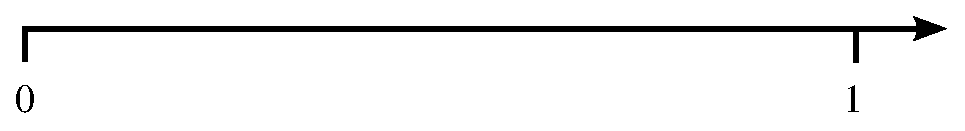
\includegraphics[width=10cm]{eps/interval.eps}
    \caption{The reference interval.}
    \label{fig:interval}
  \end{center}
\end{figure}

\begin{table}
\linespread{1.2}\selectfont
  \begin{center}
    \begin{tabular}{|c|c|}
      \hline
      Vertex & Coordinate \\
      \hline
      \hline
      $v_0$ & $x = 0$ \\
      \hline
      $v_1$ & $x = 1$ \\
      \hline
    \end{tabular}
    \caption{Vertex coordinates of the reference interval.}
    \label{tab:interval,vertices}
  \end{center}
\end{table}

\section{The reference triangle}
\index{triangle}

The reference triangle is shown in Figure~\ref{fig:triangle} and is
defined by its three vertices with coordinates as specified in
Table~\ref{tab:triangle,vertices}.

\begin{figure}
  \begin{center}
    \psfrag{v0}{$(0, 0)$}
    \psfrag{v1}{$(1, 0)$}
    \psfrag{v2}{$(0, 1)$}
    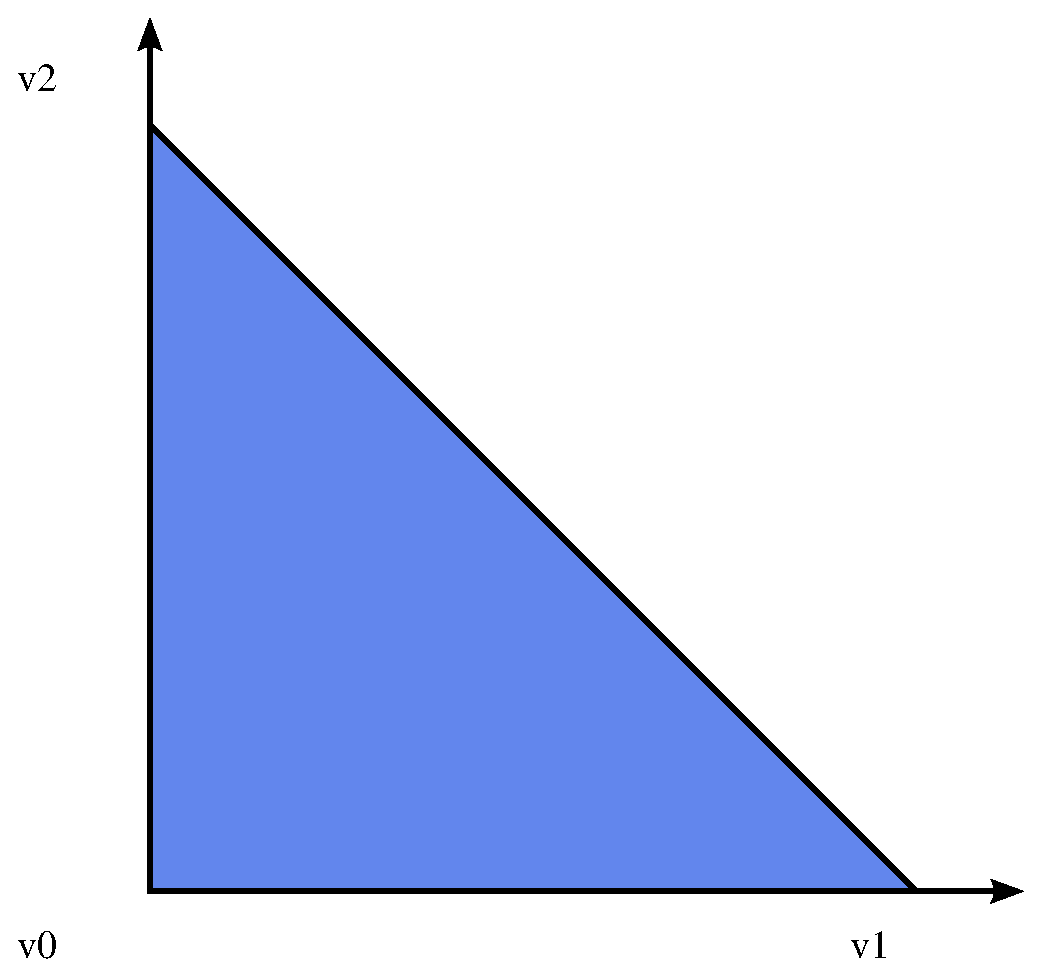
\includegraphics[width=8cm]{eps/triangle.eps}
    \caption{The reference triangle.}
    \label{fig:triangle}
  \end{center}
\end{figure}

\begin{table}
\linespread{1.2}\selectfont
  \begin{center}
    \begin{tabular}{|c|c|}
      \hline
      Vertex & Coordinate \\
      \hline
      \hline
      $v_0$ & $x = (0, 0)$ \\
      \hline
      $v_1$ & $x = (1, 0)$ \\
      \hline
      $v_2$ & $x = (0, 1)$ \\
      \hline
    \end{tabular}
    \caption{Vertex coordinates of the reference triangle.}
    \label{tab:triangle,vertices}
  \end{center}
\end{table}

\section{The reference quadrilateral}
\index{quadrilateral}

The reference quadrilateral is shown in Figure~\ref{fig:quadrilateral}
and is defined by its four vertices with coordinates as specified in
Table~\ref{tab:quadrilateral,vertices}.

\begin{figure}
  \begin{center}
    \psfrag{v0}{$(0, 0)$}
    \psfrag{v1}{$(1, 0)$}
    \psfrag{v2}{$(1, 1)$}
    \psfrag{v3}{$(0, 1)$}
    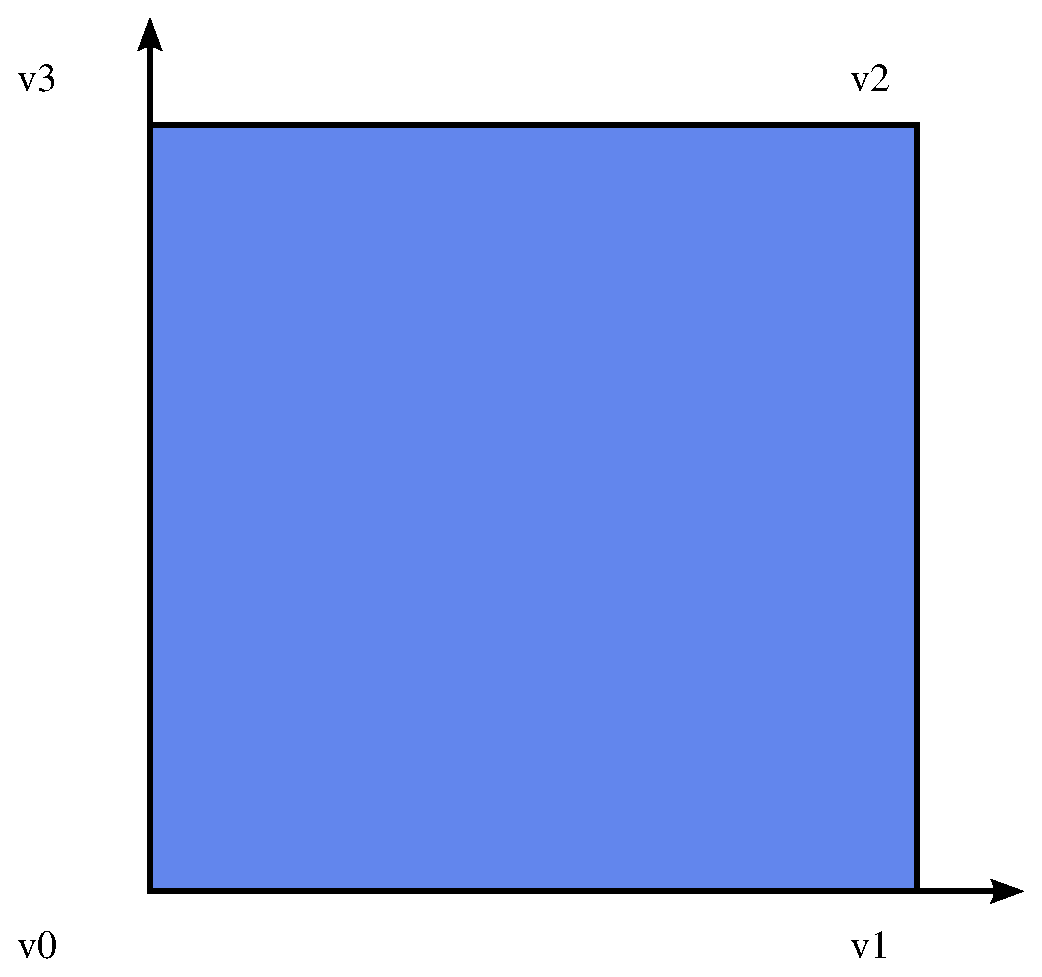
\includegraphics[width=8cm]{eps/quadrilateral.eps}
    \caption{The reference quadrilateral.}
    \label{fig:quadrilateral}
  \end{center}
\end{figure}

\begin{table}
\linespread{1.2}\selectfont
  \begin{center}
    \begin{tabular}{|c|c|}
      \hline
      Vertex & Coordinate \\
      \hline
      \hline
      $v_0$ & $x = (0, 0)$ \\
      \hline
      $v_1$ & $x = (1, 0)$ \\
      \hline
      $v_2$ & $x = (1, 1)$ \\
      \hline
      $v_3$ & $x = (0, 1)$ \\
      \hline
    \end{tabular}
    \caption{Vertex coordinates of the reference quadrilateral.}
    \label{tab:quadrilateral,vertices}
  \end{center}
\end{table}

\section{The reference tetrahedron}
\index{tetrahedron}

The reference tetrahedron is shown in Figure~\ref{fig:tetrahedron} and
is defined by its four vertices with coordinates as specified in
Table~\ref{tab:tetrahedron,vertices}.

\begin{figure}
  \begin{center}
    \psfrag{v0}{$(0, 0, 0)$}
    \psfrag{v1}{$(1, 0, 0)$}
    \psfrag{v2}{$(0, 1, 0)$}
    \psfrag{v3}{$(0, 0, 1)$}
    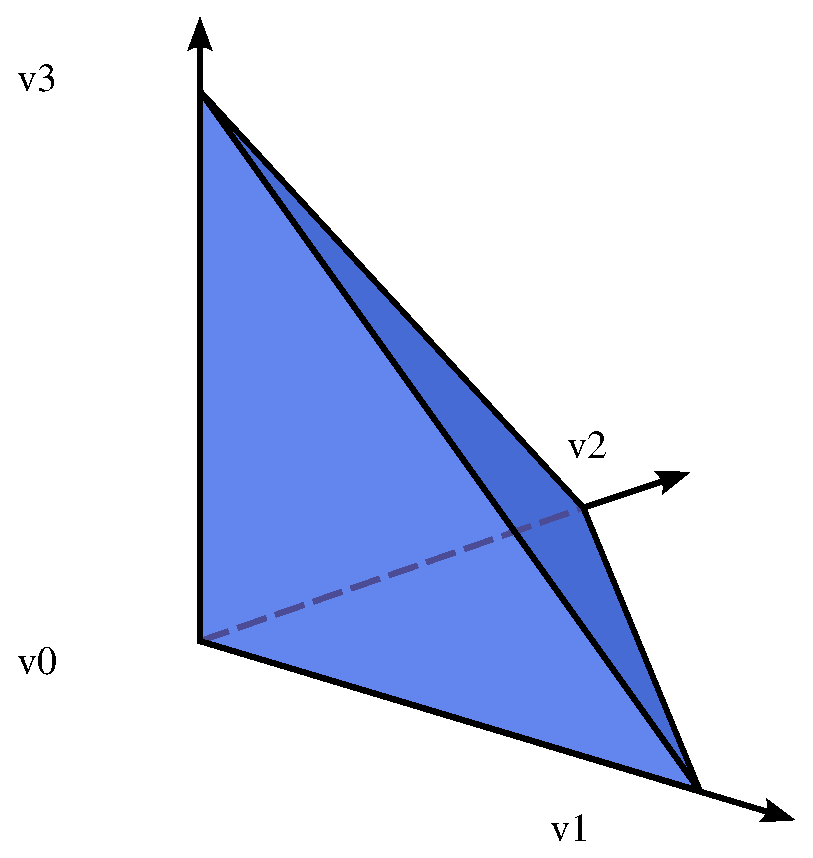
\includegraphics[width=6cm]{eps/tetrahedron.eps}
    \caption{The reference tetrahedron.}
    \label{fig:tetrahedron}
  \end{center}
\end{figure}

\begin{table}
\linespread{1.2}\selectfont
  \begin{center}
    \begin{tabular}{|c|c|}
      \hline
      Vertex & Coordinate \\
      \hline
      \hline
      $v_0$ & $x = (0, 0, 0)$ \\
      \hline
      $v_1$ & $x = (1, 0, 0)$ \\
      \hline
      $v_2$ & $x = (0, 1, 0)$ \\
      \hline
      $v_3$ & $x = (0, 0, 1)$ \\
      \hline
    \end{tabular}
    \caption{Vertex coordinates of the reference tetrahedron.}
    \label{tab:tetrahedron,vertices}
  \end{center}
\end{table}

\section{The reference hexahedron}
\index{hexahedron}

The reference hexahedron is shown in Figure~\ref{fig:hexahedron} and
is defined by its eight vertices with coordinates as specified in
Table~\ref{tab:hexahedron,vertices}.

\begin{figure}
\linespread{1.2}\selectfont
  \begin{center}
    \psfrag{v0}{$(0, 0, 0)$}
    \psfrag{v1}{$(1, 0, 0)$}
    \psfrag{v2}{$(1, 1, 0)$}
    \psfrag{v3}{$(0, 1, 0)$}
    \psfrag{v4}{$(0, 0, 1)$}
    \psfrag{v5}{$(1, 0, 1)$}
    \psfrag{v6}{$(1, 1, 1)$}
    \psfrag{v7}{$(0, 1, 1)$}
    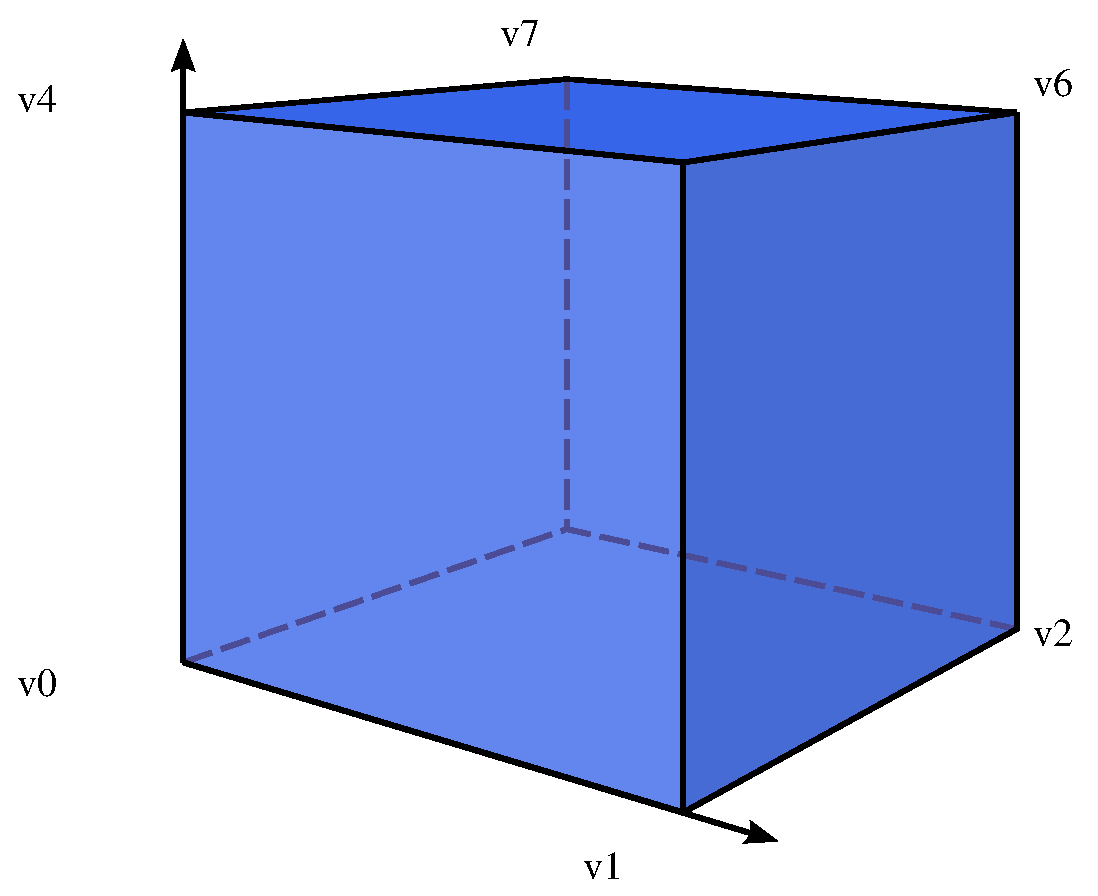
\includegraphics[width=9cm]{eps/hexahedron.eps}
    \caption{The reference hexahedron.}
    \label{fig:hexahedron}
  \end{center}
\end{figure}

\begin{table}
\linespread{1.2}\selectfont
  \begin{center}
    \begin{tabular}{|c|c|}
      \hline
      Vertex & Coordinate \\
      \hline
      \hline
      $v_0$ & $x = (0, 0, 0)$ \\
      \hline
      $v_1$ & $x = (1, 0, 0)$ \\
      \hline
      $v_2$ & $x = (1, 1, 0)$ \\
      \hline
      $v_3$ & $x = (0, 1, 0)$ \\
      \hline
    \end{tabular}
    \begin{tabular}{|c|c|}
      \hline
      Vertex & Coordinate \\
      \hline
      \hline
      $v_4$ & $x = (0, 0, 1)$ \\
      \hline
      $v_5$ & $x = (1, 0, 1)$ \\
      \hline
      $v_6$ & $x = (1, 1, 1)$ \\
      \hline
      $v_7$ & $x = (0, 1, 1)$ \\
      \hline
    \end{tabular}
    \caption{Vertex coordinates of the reference hexahedron.}
    \label{tab:hexahedron,vertices}
  \end{center}
\end{table}


\chapter{Numbering of mesh entities}

The numbering of mesh entities used in DOLFIN follows the
UFC specification~\cite{www:UFC} for each mesh that has been ordered.\footnote{To order a mesh, call the \texttt{order()} function: \texttt{mesh.order()}.}
\input{chapters/numbering_common}

\chapter{Design}

This chapter discusses details of the design of \dolfin{} and is
intended mainly for developers of \dolfin{}.

\section{Linear algebra}

The linear algebra library provides a uniform interface to uBLAS
and PETSc linear algebra through a set of wrappers for basic data
structures (matrices and vectors) and solvers, such as Krylov subspace
solvers with preconditioners.

For both sets of wrappers, a common interface is defined by the
classes \texttt{GenericMatrix} and \texttt{GenericVector}. \dolfin{}
provides a number of algorithms, most notably the assembly algorithms,
that work only through the common interface, which means that these
algorithms work for any given representation that implements the
interface specified by \texttt{GenericMatrix} or
\texttt{GenericVector}. A class diagram for the \dolfin{} linear
algebra implementation is given in Figure~\ref{fig:laclasses}.

\begin{figure}[htbp]
  \begin{center}
    \includegraphics[width=0.95\textwidth]{eps/class-diagram-la.eps}
    \caption{Class diagram of the linear algebra classes in \dolfin{}.}
    \label{fig:laclasses}
  \end{center}
\end{figure}


\input{chapters/installation.tex}
% This chapter is common to the DOLFIN and FFC manuals.

\chapter{Contributing code}
\index{contributing}

If you have created a new module, fixed a bug somewhere, or have made
a small change which you want to contribute to \package{}, then the
best way to do so is to send us your contribution in the form of a
patch. A patch is a file which describes how to transform a file or
directory structure into another. The patch is built by comparing a
version which both parties have against the modified version which
only you have. Patches can be created with Mercurial
or \texttt{diff}.

%------------------------------------------------------------------------------
\section{Creating bundles/patches}
%------------------------------------------------------------------------------
\subsection{Creating a Mercurial (hg) bundle}
\index{hg}
\index{Mercurial}
\index{bundle}

Creating bundles is the preferred way of submitting patches. It has
several advantages over plain diffs. If you are a frequent
contributor, consider publishing your source tree so that the \ffc{}
maintainers (and other users) may pull your changes directly from your
tree.

A bundle contains your contribution to \package{} in the form of a 
binary patch file  generated by Mercurial~\cite{www:Mercurial},  
the revision control system used by \package{}. 
Follow the procedure described below to create your bundle.
\begin{enumerate}
\item
  Clone the \package{} repository:
  \begin{macrocode}
# hg clone http://www.fenics.org/hg/\packagett{}
  \end{macrocode}
\item \label{label:AddFilesHg} If your contribution consists of new files, 
  add them to the 
  correct location in the \package{} directory tree. Enter the \package{}
  directory and add these files to the local repository by typing:
  \begin{macrocode}
# hg add <files>
  \end{macrocode}
  where \texttt{<files>} is the list of new files.
  You do not have to take any action for previously existing files 
  which have been modified. Do not add temporary or binary files. 
\item Enter the \package{} directory and commit your contribution:
  \begin{macrocode}
# hg commit -m "<description>"
  \end{macrocode}
  where \texttt{<description>} is a short description of what 
  your patch accomplishes.
\item Create the bundle:
  \begin{macrocode}
# hg bundle \packagett{}-<identifier>-<date>.hg 
  http://www.fenics.org/hg/\packagett{}
  \end{macrocode}
  written as one line, where \texttt{<identifier>} is a keyword that
  can be used to identify the bundle as coming from you (your username,
  last name, first name, a nickname etc) and \texttt{<date>} is
  today's date in the format \texttt{yyyy-mm-dd}.\\
  The bundle now exists as \texttt{\packagett{}-<identifier>-<date>.hg}.
\end{enumerate}

When you add your contribution at point~\ref{label:AddFilesHg}, 
make sure that only the files 
that you want to share are present by typing:
\begin{macrocode}
# hg status 
\end{macrocode}
This will produce a list of files. Those marked with a question mark 
are not tracked by Mercurial. You can track them by using the
\texttt{add}  command as shown above. Once you have 
added these files, their status changes form  \texttt{?} to \texttt{A}.
  
  
%------------------------------------------------------------------------------
\subsection{Creating a standard (diff) patch file}
\index{diff}
\index{patch}

The tool used to create a patch is called \texttt{diff} and the tool
used to apply the patch is called \texttt{patch}.

Here's an example of how it works. Start from the latest release of
\package{}, which we here assume is release x.y.z. You then have a
directory structure under \texttt{\packagett{}-x.y.z} where you have made
modifications to some files which you think could be useful to
other users.

\begin{enumerate}
\item
  Clean up your modified directory structure to remove temporary and binary
  files which will be rebuilt anyway:
  \begin{code}
# make clean
  \end{code}
\item
  From the parent directory, rename the \package{} directory to something else:
  \begin{macrocode}
# mv \packagett{}-x.y.z \packagett{}-x.y.z-mod
  \end{macrocode}
\item
  Unpack the version of \package{} that you started from:
  \begin{macrocode}
# tar zxfv \packagett{}-x.y.z.tar.gz
  \end{macrocode}
\item
  You should now have two \package{} directory structures in your current directory:
  \begin{macrocode}
# ls
\packagett{}-x.y.z
\packagett{}-x.y.z-mod
  \end{macrocode}
\item
  Now use the \texttt{diff} tool to create the patch:
  \begin{macrocode}
# diff -u --new-file --recursive \packagett{}-x.y.z
  \packagett{}-x.y.z-mod > \packagett{}-<identifier>-<date>.patch
  \end{macrocode}
  written as one line, where \texttt{<identifier>} is a keyword that
  can be used to identify the patch as coming from you (your username,
  last name, first name, a nickname etc) and \texttt{<date>} is
  today's date in the format \texttt{yyyy-mm-dd}.
\item
  The patch now exists as \texttt{\packagett{}-<identifier>-<date>.patch}
  and can be distributed to other people who already have
  \texttt{\packagett{}-x.y.z} to easily create your modified version. If the
  patch is large, compressing it with for example \texttt{gzip} is
  advisable:
  \begin{macrocode}
# gzip \packagett{}-<identifier>-<date>.patch
  \end{macrocode}
\end{enumerate}

%------------------------------------------------------------------------------
\section{Sending bundles/patches}
\index{patch}
\index{bundle}

Patch and bundle files should be sent to the \package{} mailing list at the address
\begin{macrocode}
\packagett{}-dev@fenics.org
\end{macrocode}
Include a short description of what your patch/bundle accomplishes. Small
patches/bundles have a better chance of being accepted, so if you are making a
major contribution, please consider breaking your changes up into
several small self-contained patches/bundles if possible.

%------------------------------------------------------------------------------
\section{Applying changes}
%------------------------------------------------------------------------------
\subsection{Applying a Mercurial bundle}
\index{bundle}
\index{hg}
\index{Mercurial}

You have received a patch in the form of a Mercurial bundle. The following
procedure shows how to apply the patch to your version of \package{}.
\begin{enumerate}
\item Before applying the patch, you can check
  its content by entering the \package{} directory and typing:
  \begin{macrocode}
# hg incoming -p 
  bundle://<path>/\packagett{}-<identifier>-<date>.hg
  \end{macrocode}
  written as one line, where \texttt{<path>} is the path to the
  bundle. \texttt{<path>} can be omitted if the bundle is in the
  \package{} directory.  The option \texttt{-p} can be omitted if you
  are only interested in a short summary of the changesets found in
  the bundle.
\item To apply the patch to your version of \package{} type:
  \begin{macrocode}
# hg unbundle <path>/\packagett{}-<identifier>-<date>.hg
  \end{macrocode}
  followed by:
  \begin{macrocode}
  # hg update
  \end{macrocode}
\end{enumerate}

%------------------------------------------------------------------------------
\subsection{Applying a standard patch file}
\index{patch}

Let's say that a patch has been built relative to \package{} release x.y.z.
The following description then shows how to apply the patch to a clean
version of release x.y.z.

\begin{enumerate}
\item
  Unpack the version of \package{} which the patch is built relative to:
  \begin{macrocode}
# tar zxfv \packagett{}-x.y.z.tar.gz
  \end{macrocode}
\item
  Check that you have the patch \texttt{\packagett{}-<identifier>-<date>.patch} and the \package{}
  directory structure in the current directory:
  \begin{macrocode}
# ls
\packagett{}-x.y.z
\packagett{}-<identifier>-<date>.patch
  \end{macrocode}
  Unpack the patch file using \texttt{gunzip} if necessary.
\item
  Enter the \package{} directory structure:
  \begin{macrocode}
# cd \packagett{}-x.y.z
  \end{macrocode}
\item
  Apply the patch:
  \begin{macrocode}
# patch -p1 < ../\packagett{}-<identifier>-<date>.patch
  \end{macrocode}
  The option \texttt{-p1} strips the leading directory from the filename
  references in the patch, to match the fact that we are applying the
  patch from inside the directory. Another useful option to
  \texttt{patch} is \texttt{--dry-run} which can be used to test the
  patch without actually applying it.
\item
  The modified version now exists as \texttt{\packagett{}-x.y.z}.
\end{enumerate}

% DOLFIN-specific part of chapter contributing.tex

%------------------------------------------------------------------------------
\section{License agreement}
\index{license}

By contributing a patch to \package{}, you agree to license your
contributed code under the GNU General Public License (a condition
also built into the GPL license of the code you have modified). Before
creating the patch, please update the author and date information of
the file(s) you have modified according to the following example:

\begin{code}
  // Copyright (C) 2004-2005 Johan Hoffman and Anders Logg.
  // Licensed under the GNU GPL Version 2.
  //
  // Modified by Johan Jansson 2005.
  // Modified by Garth N. Wells 2005.
  //
  // First added:  2004-06-22
  // Last changed: 2005-09-01
\end{code}

As a rule of thumb, the original author of a file holds the copyright.

\chapter{Contributors}

\devnote{List all contributors here.}
\chapter{Coding style}
\label{sec:codingstyle}
\index{coding style}

To streamline the \dolfin{} source code and ease the job for
maintainers that need to read and edit large amounts of code,
developers should try to follow the below coding style when submitting
patches to \dolfin{}.

The guideline below is for C++ but may in some cases be extrapolated
to Python.

\section{Naming conventions}

\subsection{Class names}

Use camel caps for class names:
\begin{code}
class FooBar
{
  ...
};
\end{code}

\subsection{Function names}

Use lower-case for function names and underscore to separate words:
\begin{code}
void foo();
void bar();
void foo_bar(...);
\end{code}

Functions returning a value should be given the name of that value,
for example:
\begin{code}
class Array:
{
public:

  /// Return size of array (number of entries)
  uint size() const;

};
\end{code}

In the above example, the function should be named \texttt{size} rather
than \texttt{get\_size}. On the other hand, a function not returning a
value but rather taking a variable (by reference) and assigning a value
to it, should use the \texttt{get\_foo} naming scheme, for example:
\begin{code}
class Parameters:
{
public:

  /// Retrieve all parameter keys
  void get_parameter_keys(std::vector<std::string>& parameter_keys) const;

};
\end{code}

\subsection{Variable names}

Use lower-case for variable names and underscore to separate words:
\begin{code}
Foo foo;
Bar bar;
FooBar foo_bar;
\end{code}

\subsection{Enum variables and constants}

Enum variables should be lower-case with underscore to separate words:
\begin{code}
enum Type {foo, bar, foo_bar};
\end{code}

We try to avoid using \texttt{\#define} to define constants, but when
necessary constants should be capitalized:
\begin{code}
#define FOO 3.14159265358979
\end{code}

\subsection{File names}

Use camel caps for file names if they contain the
declaration/definition of a class. Header files should have the
suffix~\texttt{.h} and implementation files should have the
suffix~\texttt{.cpp}:
\begin{code}
FooBar.h
FooBar.cpp
\end{code}

Use lower-case for file names that contain utilities/functions (not
classes).

\section{Miscellaneous}

\subsection{Comments}

Comment your code, and do it often. Capitalize the first letter and
don't use punctuation (unless the comment runs over several
sentences). Here's a good example from \texttt{TopologyComputation.cpp}:
\begin{code}
// Check if connectivity has already been computed
if (connectivity.size() > 0)
  return;

// Invalidate ordering
mesh._ordered = false;

// Compute entities if they don't exist
if (topology.size(d0) == 0)
  computeEntities(mesh, d0);
if (topology.size(d1) == 0)
  computeEntities(mesh, d1);

// Check if connectivity still needs to be computed
if (connectivity.size() > 0)
  return;

...
\end{code}

\subsection{Integers and reals}

Use \texttt{dolfin::uint} instead of \texttt{int} (unless you really
want to use negative integers which is rare) and \texttt{dolfin::real}
instead of \texttt{double}:
\begin{code}
uint i = 0;
double x = 0.0;
\end{code}
These are typedefs for the standard C++ types \texttt{unsigned int}
and \texttt{double} (defined in \texttt{dolfin/common/types.h}).

\subsection{Placement of brackets}

Curly brackets following a control statement should appear in the next
line and not be indented:
\begin{code}
for (uint i = 0; i < 10; i++)
{
  ...
}
\end{code}

\subsection{Indentation}

Indentation should be two spaces and it should be spaces, \emph{not}
tab(s).

\subsection{Header file layout}

Header files should follow the below template:
\vspace{-0.5cm}
\begin{code}
// Copyright (C) 2008 Foo Bar.
// Licensed under the GNU LGPL Version 2.1.
//
// Modified by Bar Foo, 2008.
//
// First added:  2008-01-01
// Last changed: 2008-02-01

#ifndef __FOO_H
#define __FOO_H

namespace dolfin
{

  class Bar; // Forward declarations here

  /// Documentation of class

  class Foo
  {
  public:

    ...

  private:

    ...

  };

}

#endif
\end{code}

\subsection{Implementation file layout}

Implementation files should follow the below template:
\begin{code}
// Copyright (C) 2008 Foo Bar.
// Licensed under the GNU LGPL Version 2.1.
//
// Modified by Bar Foo, 2008.
//
// First added:  2008-01-01
// Last changed: 2008-02-01

#include <dolfin/Foo.h>

using namespace dolfin;

//-----------------------------------------------------------
Foo::Foo() : // variable initialization here
{
  ...
}
//-----------------------------------------------------------
Foo::~Foo()
{
  // Do nothing
}
//-----------------------------------------------------------
\end{code}

The horizontal lines above should be exactly~79 characters
wide but have been shortened here to fit the page.

\subsection{Including header files}

Don't use \texttt{\#include <dolfin.h>} or \texttt{\#include
  <dolfin/dolfin\_foo.h>} inside the DOLFIN kernel. Only include the
portions of DOLFIN you are actually using.

\subsection{Forward declarations}

Actually, try to include as little as possible and use forward
declarations whenever possible (in header files). Put the
\texttt{\#include} in the implementation file.

\subsection{Explicit constructors}

Make all constructors (except copy constructors) explicit if there is no particular
reason not to do so:
\begin{code}
class Foo
{
  explicit Foo(uint i);
};
\end{code}

\input{chapters/license.tex}

\end{document}
